\documentclass{article}

\usepackage{algorithmic}
\usepackage{amsmath}
\usepackage{graphicx}
\usepackage{hyperref}
\usepackage{booktabs}

\begin{document}

\title{Final Exam}
\author{Geoffrey Ulman\\
        CSI873}
\date{December 2011}
\maketitle

\section{Results}\label{Results}

\begin{figure}
\centering
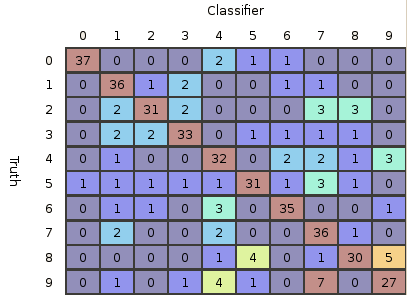
\includegraphics[width=0.9\textwidth]{images/poly_all_confusion_test.png}
\caption{Polynomial Kernel 10 Digit Test Error Confusion Matrix}
\label{poly10testconfusion}
\end{figure}

\begin{figure}
\centering
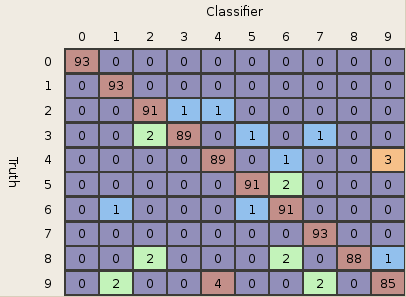
\includegraphics[width=0.9\textwidth]{images/poly_all_confusion_training.png}
\caption{Polynomial Kernel 10 Digit Training Error Confusion Matrix}
\label{poly10trainconfusion}
\end{figure}

\begin{figure}
\centering
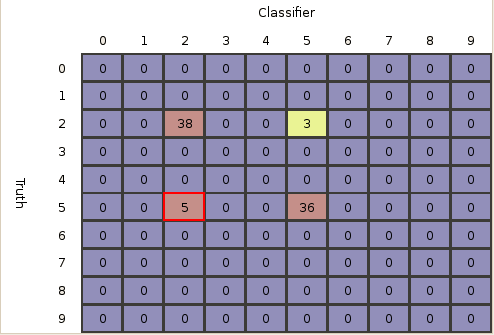
\includegraphics[width=0.9\textwidth]{images/test2_5_confusion_a0156.png}
\caption{Polynomial Kernel 2 Digit Test Error Confusion Matrix}
\label{poly2testconfusion}
\end{figure}

\begin{figure}
\centering
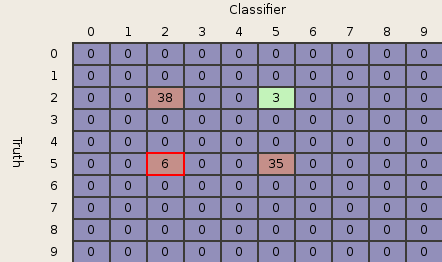
\includegraphics[width=0.9\textwidth]{images/test2_5_confusion_radial.png}
\caption{Radial Kernel 2 Digit Test Error Confusion Matrix}
\label{radial2testconfusion}
\end{figure}

\begin{figure}
\centering
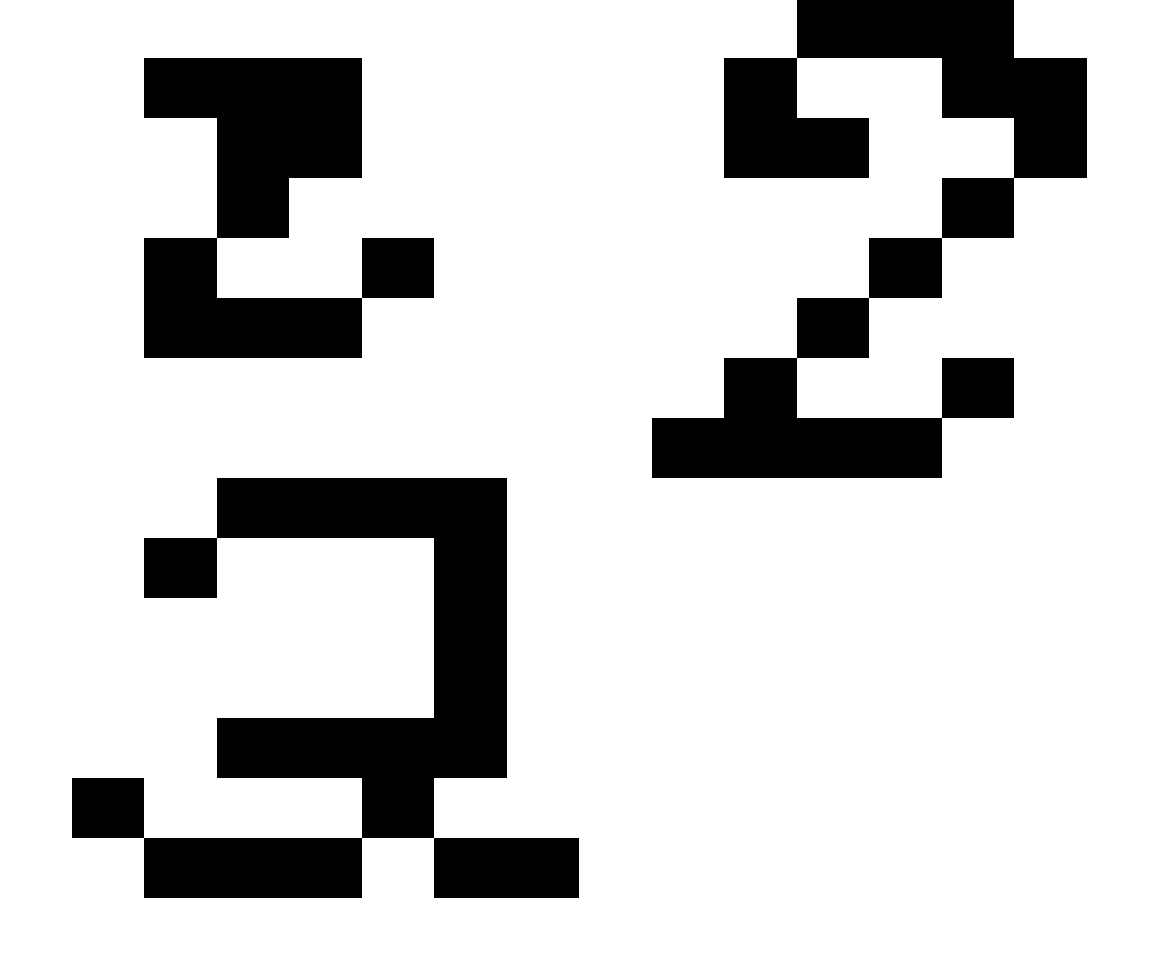
\includegraphics[width=0.9\textwidth]{images/test2_5_correct2_class5_a0156.png}
\caption{Polynomial Kernel 2 Missclassified as 5}
\label{poly2errortest}
\end{figure}

\begin{figure}
\centering
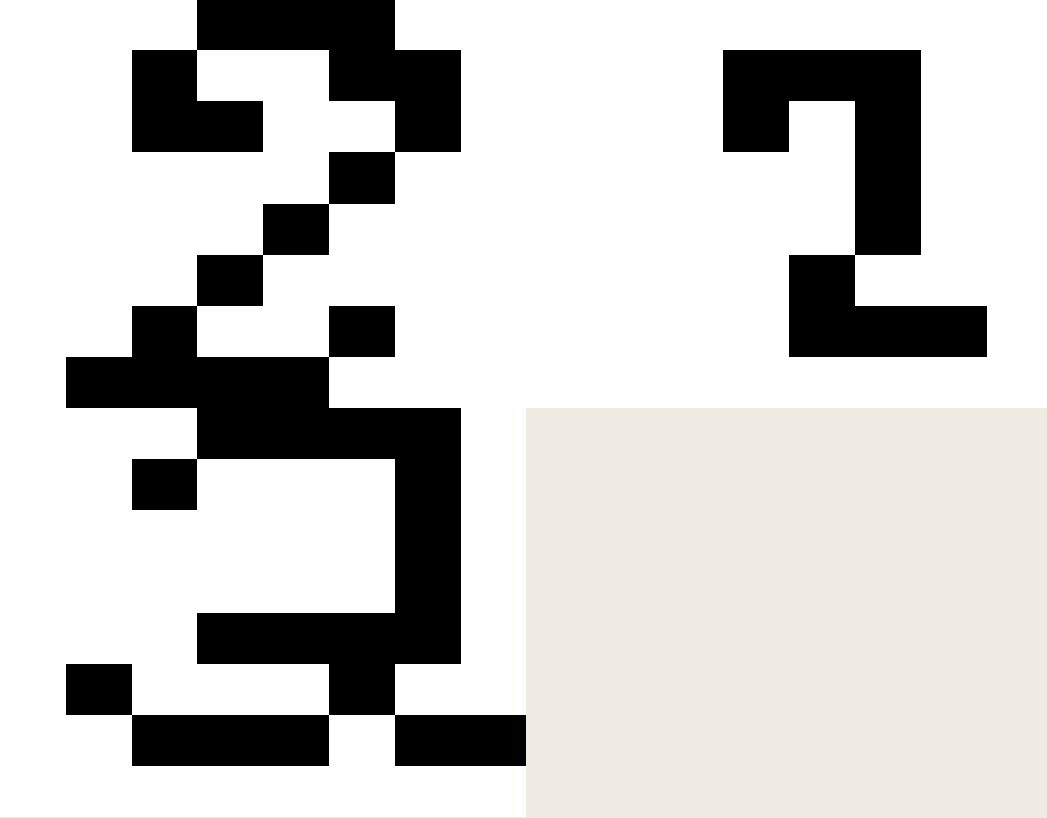
\includegraphics[width=0.9\textwidth]{images/test2_5_correct2_class5_radial.png}
\caption{Radial Kernel 2 Missclassified as 5}
\label{radial2errortest}
\end{figure}

\begin{figure}
\centering

\includegraphics[width=0.9\textwidth]{images/test2_5_correct5_class2_a0156.png}
\caption{Polynomial Kernel 5 Missclassified as 2}
\label{poly5errortest}
\end{figure}

\begin{figure}
\centering
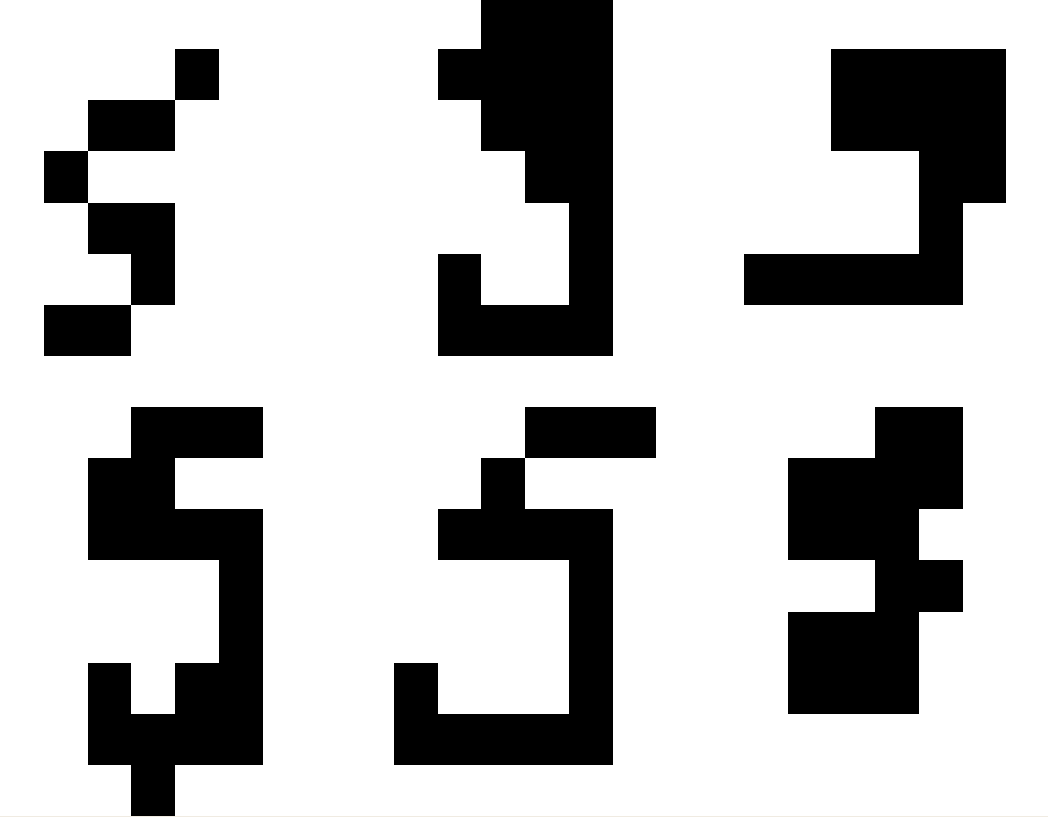
\includegraphics[width=0.9\textwidth]{images/test2_5_correct5_class2_radial.png}
\caption{Radial Kernel 5 Missclassified as 2}
\label{radial5errortest}
\end{figure}

\begin{figure}
\centering
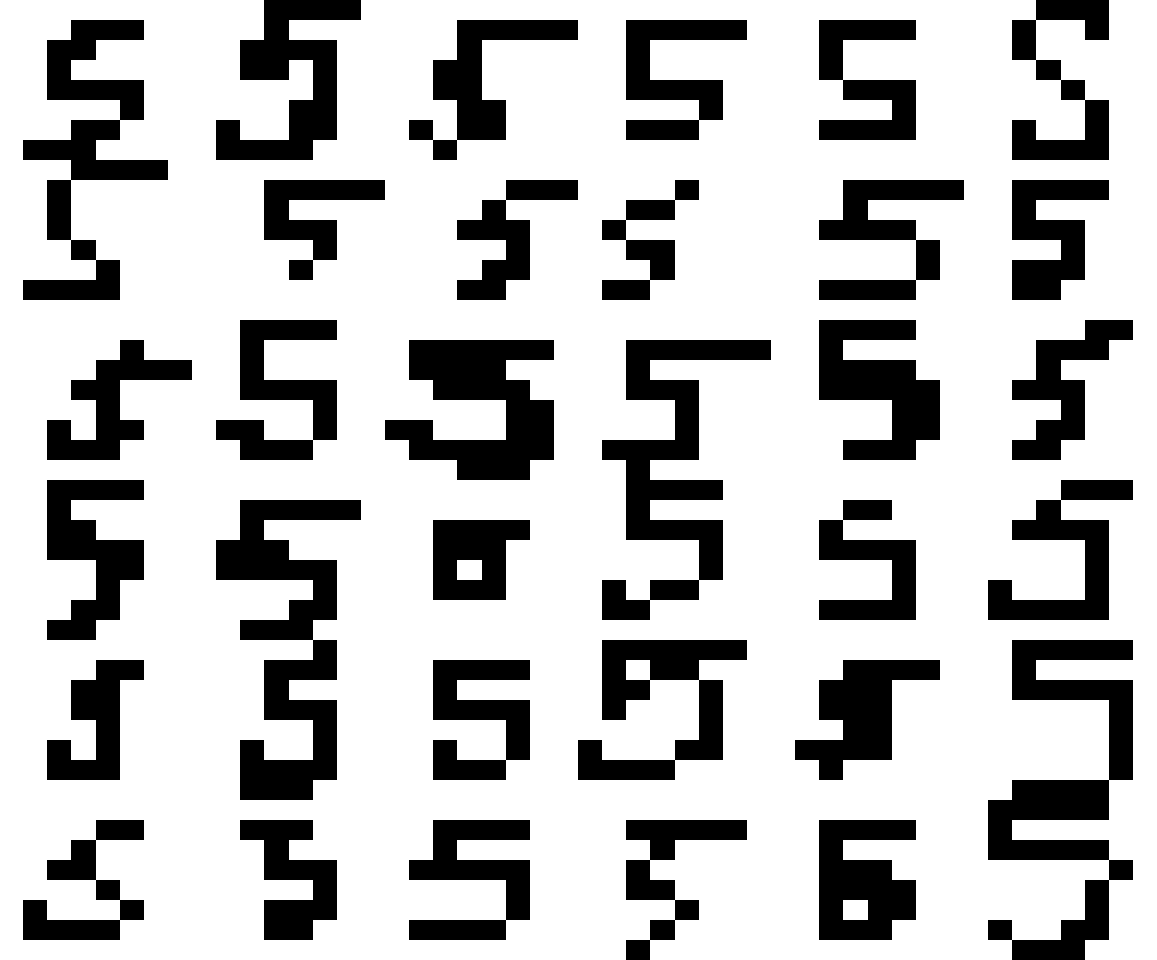
\includegraphics[width=0.9\textwidth]{images/test2_5_correct5s_a0156.png}
\caption{Polynomial Kernel Correctly Classified 5 Digits}
\label{poly5correcttest}
\end{figure}

\begin{figure}
\centering
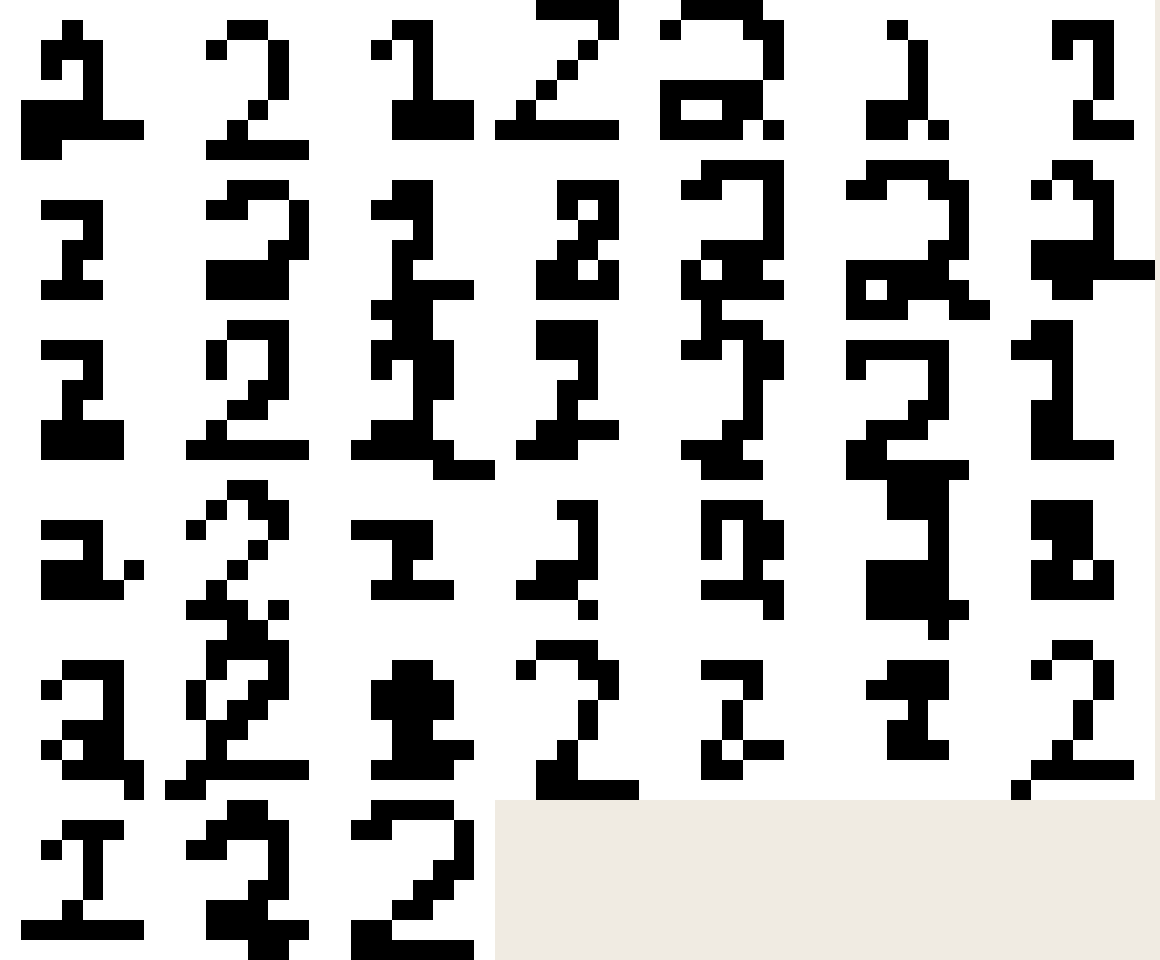
\includegraphics[width=0.9\textwidth]{images/test2_5_correct2s_a0156.png}
\caption{Polynomial Kernel Correctly Classified 2 Digits}
\label{poly2correcttest}
\end{figure}

\begin{figure}
\centering
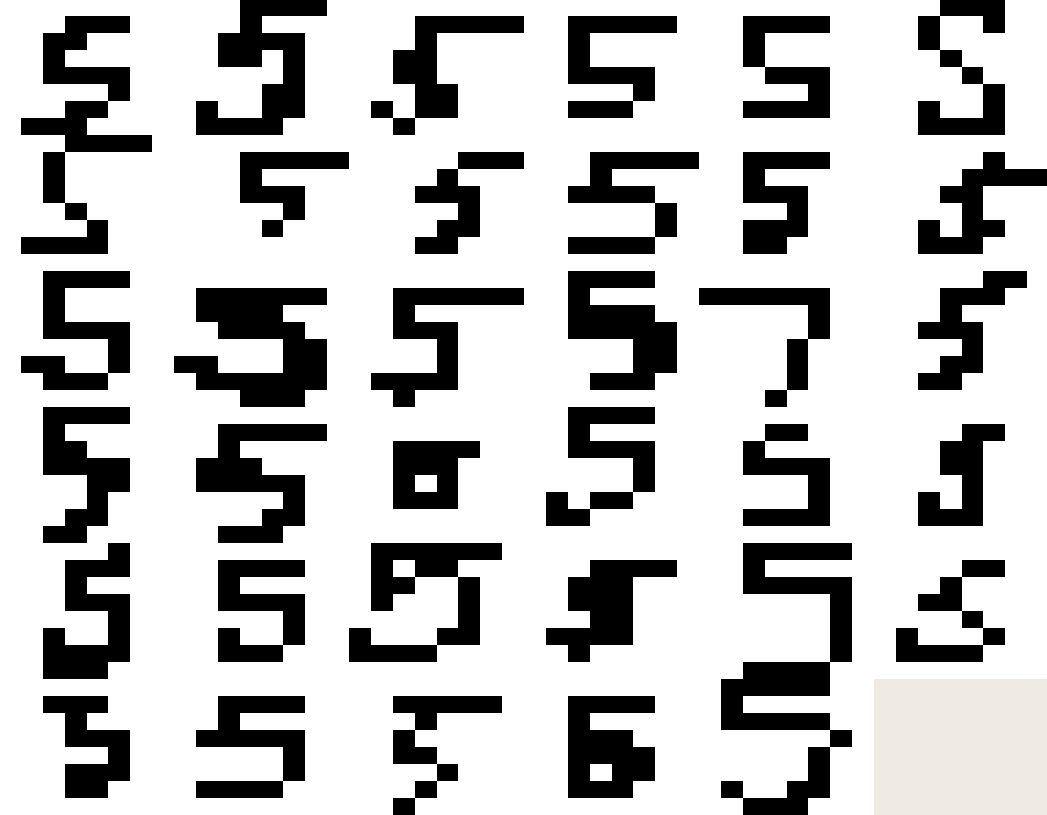
\includegraphics[width=0.9\textwidth]{images/test2_5_correct5_radial.png}
\caption{Radial Kernel Correctly Classified 5 Digits}
\label{radial5correcttest}
\end{figure}

\begin{figure}
\centering
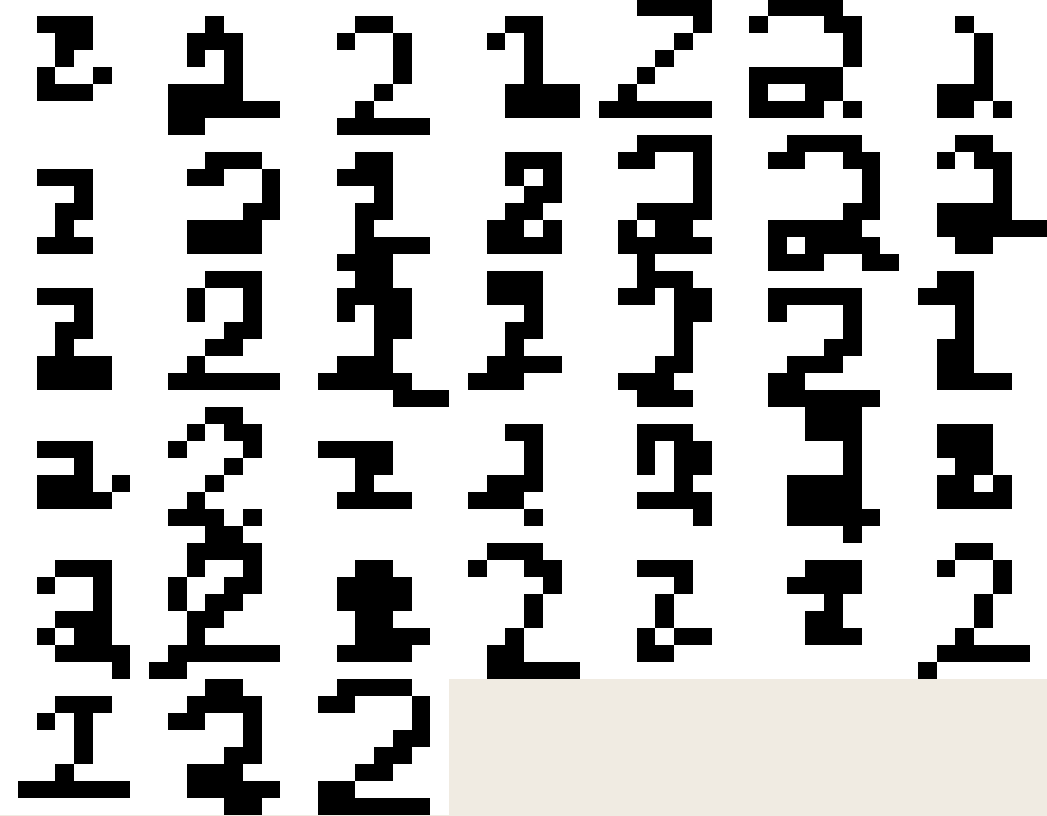
\includegraphics[width=0.9\textwidth]{images/test2_5_correct2_radial.png}
\caption{Radial Kernel Correctly Classified 2 Digits}
\label{radial2correcttest}
\end{figure}

\begin{thebibliography}{9}

\bibitem{cpl}
  Tom M. Mitchell,
  \emph{Machine Learning},
  WCB McGraw-Hill, Boston,
  1997.

\end{thebibliography}

\end{document}
